\chapter{Boomerang Plans}


The following descriptions indicate characteristics and options for the boomerangs which can be adopted when constructing these boomerangs. For further details see previous chapters.

\newpage
\section{Standard}
\begin{tabulary}{30em}{>{\bfseries}lL}
Shape:							& Michael Siems (Germany) \\
Use: 								& Boomerang for beginners\\
Flight distance:	 		& approx. 20 metres\\ 
Thickness/material:		& 4-5 mm finnish birch plywood\\
Weight: 						& 80 g / 2.85 oz. \vspace{0.5em} \\
Airfoil: 							& 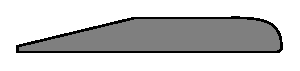
\includegraphics[width=18em]{Pictures/80_PRO1.eps} \vspace{0.5em} \\
Underside:					& Try a slight undercut on both arms.\\
Tuning: 						& Slight positive dihedral on both arms.\\
Wind:							& 0 - 2 Beaufort\\
\end{tabulary}

\vspace*{\fill}
\begin{center}
	
\includegraphics[ angle=90, width=0.72\textwidth]{plans/Standard.eps} 
\end{center}
\vspace{\fill}


\section{Outback II}
\begin{tabulary}{30em}{>{\bfseries}lL}
Shape: 							& Doug DuFresne (USA) \\
Use: 								& Boomerang for beginners, Trick Catching \\
Flight distance: 			& approx. 20 - 30 metres \\
Thickness/material: 	& 4 - 5 mm finnish birch plywood \\
Weight: 						& 75 g / 2.7 oz.  \vspace{0.5em} \\

Airfoil:							& 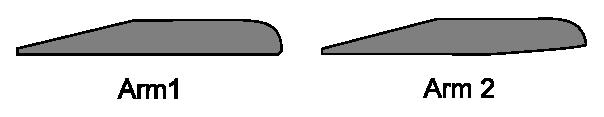
\includegraphics[width=18em]{Pictures/81_PRO2.eps} \vspace{0.5em} \\
         
Underside:					& Pronounced undercut on arm 2 from elbow to wing tip.\\
Wind:							& 0 - 2 Beaufort\\
\end{tabulary}
\newpage

\vspace*{\fill}
\begin{center}
	
\includegraphics[width=\textwidth]{plans/OutbackII.eps} 
\end{center}
\vspace{\fill}
\newpage

\section{Bellen}
\begin{tabulary}{30em}{>{\bfseries}lL}
Shape:							& Michael ``Gel'' Girvin (USA)\\
Use:								& Boomerang for beginners, Trick Catching, Accuracy, Juggling \\
Flight distance: 			& Approx. 20 metres \\
Weight: 						& 72 g / 2.6 oz. \\
Thickness/material: 	& 4 - 5 mm finnish birch plywood \vspace{0.5em} \\
Airfoil:							& 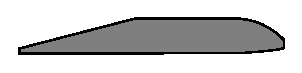
\includegraphics[width=18em]{Pictures/82_PRO3.eps} \vspace{0.5em} \\
Underside:					& Try a slight undercut on both arms\\
Wind:							& 0 - 3 Beaufort\\
Special features:			& John Flynn and Michael „Gel“ Girvin both held the world record in Juggling with „Bellens“\\
\end{tabulary}
\newpage

\vspace*{\fill}
\begin{center}
	
\includegraphics[angle=-90, width=28em]{plans/Bellen.eps}
\end{center}
\vspace{\fill}
\newpage

\section{Carlota}
\begin{tabulary}{30em}{>{\bfseries}lL}
Shape:							& Michael ``Gel'' Girvin (USA)\\
Use:								& Trick Catch, Juggling, Doubling \\
Flight distance:			& Approx. 20 metres \\
Thickness/material:		& 3 - 4 mm finnish birch plywood \\
Weight:							& ?? g / ?? oz.\vspace{0.5em} \\
Airfoil:							& 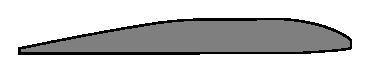
\includegraphics[width=18em]{Pictures/83_PRO4.eps} \vspace{0.5em} \\
Holes:							& There should be holes on the ends of a pair of doublers. \\
Wind:							& 0 - 3 Beaufort\\
Special features:			& Two Carlotas, as similar as possible, should be used for Juggling. A rubberband can be added to the center to stabilize hover.\\
\end{tabulary}
\newpage

\vspace*{\fill}
\begin{center}
	
\includegraphics[angle=0,width=\textwidth]{plans/Carlotta.eps}
\end{center}
\vspace{\fill}


\newpage
\section{Fuzzy}
\begin{tabulary}{30em}{>{\bfseries}lL}
Shape:							& Axel Heckner (Germany)\\
Use:								& Trick catching, Accuracy, Fast Catch, Australian Round \\
Flight distance:			& Approx. 20 - 50 m, depending on the features\\
Thickness/material: 	& 4 mm finnish birch plywood \\
Weight:							& Between 35 g / 1.25 oz and  70 g / 2.5 oz. \vspace{0.5em} \\
Airfoil:							& 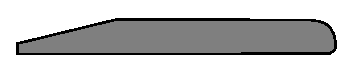
\includegraphics[width=18em]{Pictures/85_PRO6.eps} \vspace{0.5em} \\
Underside:					& Try slight undercut on both arms\\
Wind:							& 0 - 4 Beaufort \\
Flight path:					& Circular, flies at one level, lies flat at end of flight\\
Tips:								& Weights close to the centre of rotation make it unusually stable in wind\\
Special features:			& A very accurate return. By adjusting weights at the wing tips, it is easy to adjust the distance. Wheighted, Fuzzy can have a range of up to 50 metres\\
\end{tabulary}
\newpage

\vspace*{\fill}
\begin{center}
	
\includegraphics[angle=90, width=\textwidth]{plans/Fuzzy.eps} 
\end{center}
\vspace{\fill}

\newpage
\section{Albatros}
\begin{tabulary}{30em}{>{\bfseries}lL}
Shape:							& Michael Siems \\
Use: 								& Australian round\\ 
Flight distance: 			& 50 - 60 metres \\
Thickness/material: 	& 5 - 6 mm finnish birch plywood \\
Weight:							& 100 g / 3.6 oz. \vspace{0.5em} \\
Airfoil:							& 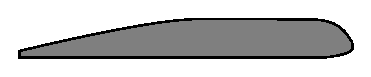
\includegraphics[width=18em]{Pictures/86_PRO7.eps} \vspace{0.5em} \\
Underside:					& Slight undercut on both arms\\
Weights:						& 10 mm diametre lead weights in both arms, in addition tape two small coins on top of arm 1 and one small coin on top of arm 2 on the middle of the airfoil\\
Tuning:						& very slight positive dihedral on both arms \\
Wind:							& 1 - 4 Beaufort\\
Throw:							& 80° angle to the wind, 30° - 45° tilt, 0°  . If there is little wind, use more tilt and angle to the wind and throw lower\\
Flight path:					& Big circle, flies fairly low\\
Tips:								& The 6 mm thick Albatros returns even if there isn’t much wind\\
\end{tabulary}
\newpage

\vspace*{\fill}
\begin{center}
	
\includegraphics[angle=90, width=28em]{plans/Albatros.eps} 
\end{center}
\vspace{\fill}

\newpage
\section{Ikarus}
\begin{tabulary}{30em}{>{\bfseries}lL}
Shape:							& Axel Heckner \\
Use:								& Australian Round \\
Flight distance:			& Approx. 50 metres\\
Thickness/material: 	& 5 - 6 mm finnish birch plywood \\
Weight: 						& 70 g / 2.5 oz. \vspace{0.5em} \\
Airfoil:							& 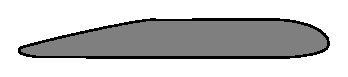
\includegraphics[width=18em]{Pictures/87_PRO8.eps} \vspace{0.5em} \\
Underside:					& An undercut on the leading- and trailing edge\\
Weights:						& With a weight on arm 1, distances of up to 80 metres can be reached. If the boomerang flies too low, put a small weight on the elbow or arm 2\\
Wind:							& 0 - 1 Beaufort, up to 4 Beaufort with a weight on arm 1 \\
Throw: 							& 80° angle to the wind, 20° - 30° tilt, 0° - 5° height of throw\\
Flight path:					& Circular, low and steady\\
Tips: 							& If it is a clumsy flight, more undercut will help on the leading edge especially on arm 2\\
Special features:			& Flies surprisingly far for a wooden boomerang and needs little wind. With a thickness of 5 mm, it can fly approx. 40 metres and needs a bit more wind\\
\end{tabulary}
\newpage

\vspace*{\fill}
\begin{center}
	
\includegraphics[width=\textwidth]{plans/Ikarus.eps} 
\end{center}
\vspace{\fill}

\newpage
\section{Eric’s Fast Catch}
\begin{tabulary}{30em}{>{\bfseries}lL}
Shape:							& Eric Darnell (USA) \\
Use:								& Fast Catch \\
Flight distance: 			& Approx. 20 metres\\
Thickness/material: 	& 4 mm finnish birch plywood or a TriFly (see Appendix on boomerang manufacturers) \\
Weight:							& 30 g / 1.1 oz. \vspace{0.5em} \\
Airfoil:							& 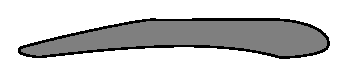
\includegraphics[width=18em]{Pictures/88_PRO9.eps} \vspace{0.5em} \\
Weights: 						& Possibly wrap tape around the wing tips ( 2 to 5 times) to reach the required distance. Holes: one to two holes (7 - 10 mm / 1/4" - 3/8") on the wing tips on all arms\\
Tuning: 						& Negative dihedral and positive angle of attack on all arms.\\
Wind: 							& 0 - 2 Beaufort\\
Throw:							& Approx 80° angle to the wind, 0° height of throw and -5° to 5° tilt \\
Flight path: 					& Circular and low\\
Tips: 							& The tuning is very important with this boomerang. 
								       By tuning you can adjust the distance and height\\
Special features: 			& Because of the holes, the boomerang must be thrown very hard (and is therefore very fast), it will return with little rotation and translation speed, but is easy to catch\\
\end{tabulary}
\newpage

\vspace*{\fill}
\begin{center}
	
\includegraphics[angle=90,width=\textwidth]{plans/EricsFastCatch.eps} 
\end{center}
\vspace{\fill}

\newpage
\section{Ice Runner II}
\begin{tabulary}{30em}{>{\bfseries}lL}
Shape:							& Fridolin Frost \\
Use: 								& Fast Catch \\
Flight distance: 			& Approx. 20 metres\\
Thickness/material: 	& 4 mm in finnish birch plywood or polypropylene\\
Weight: 						& 35 g / 1.25 oz in wood; 40 g / 1.4 oz in polypropylene \vspace{0.5em} \\
Airfoil:							& 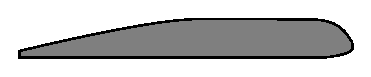
\includegraphics[width=18em]{Pictures/89_PRO10.eps} \vspace{0.5em} \\
Underside:					& Try slight undercut on all three arms\\
Weights: 						& Wrap tape around the wing tips. (1 - 3 times) in order to reach the required 20 m if necessary. \\
Throw: 							& approx. 80° angle to the wind, approx. 0° height of throw, -5 to 5 tilt\\
Wind: 							& 0 - 4 Beaufort\\
Flight path: 					& Circular, low, fast return\\
Tips: 							& Depending on the force of the throw, you might need dihedral: if it suddenly crashes to the ground, you will need positive dihedral, if it flies too high towards the end of the flight, negative dihedral is needed\\
\end{tabulary}
\newpage

\vspace*{\fill}
\begin{center}
	
\includegraphics[angle=-90, width=\textwidth]{plans/IceRunnerII.eps} 
\end{center}
\vspace{\fill}

\newpage
\section{Triller}
\begin{tabulary}{30em}{>{\bfseries}lL}
Shape:							& Axel Heckner \\
Use:								& Fast Catch \\
Flight distance:			& Approx. 20 metres \\
Thickness/material:		& 4 mm finnish birch plywood \\
Weight:							& 37 g / 1.3 oz. \vspace{0.5em} \\
Airfoil:							& 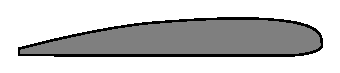
\includegraphics[width=18em]{Pictures/90_PRO11.eps} \vspace{0.5em} \\
Underside:					& Slight undercut along the whole of the airfoil, on all three arms\\
Weights:						& Wrap tape around the wing tips ( 1 - 3 times) to reach the required 20 metres distance if needed\\
Wind: 							& 0 - 1 Beaufort \\
Throw:							& Approx. 80° angle to the wind, approx. 0° height of throw, -5° - 5° tilt\\
Flight path:					& Circular, low, fast return\\
Tips:								& If the triller is too fast, it can be slowed down and wind stabilized by putting holes or flaps on the wing tips\\
Special features:			& It flies extremely fast, even with a gentle throw. If it is windy, the boomerang can be wind stabilized roughening the wing tips. and attaching small weights. Consider using gloves for catching.\\
\end{tabulary}
\newpage

\vspace*{\fill}
\begin{center}
	
\includegraphics[width=\textwidth]{plans/Triller.eps} 
\end{center}
\vspace{\fill}

\section{Floater}
\begin{tabulary}{30em}{>{\bfseries}lL}
Shape:							& Ted Bailey (USA)\\
Use:								& Maximum Time Aloft (MTA)\\
Flight distance: 			& 20 metres in wood \\
Thickness/material:		& 2 - 3 mm wood \\
Weight:							& 25 g / 0.9 oz. \vspace{0.5em} \\
Airfoil:							& 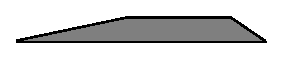
\includegraphics[width=18em]{Pictures/91_PRO12.eps} \vspace{0.5em} \\
Upper surface:				& As smooth as possible \\
Tuning:						& Arm 1: positive dihedral 6 - 10 mm; positive angle of attack 1 - 2 mm.		Arm 2: positive dihedral 2 - 5 mm; negative angle of attack 0 - 1 mm\\
Wind:							& 0 - 2 Beaufort\\
Throw:							& 5° - 10° angle to the wind, 30° - 50° height of throw, -10° - 20° tilt\\
Flight path: 					& Rises immediately and lies flat. At a height of about 10 - 30 metres it reaches the hovering phase and slowly descends with the wind\\
Remarks: 						&	It is very difficult to tune and throw an MTA boomerang. Beginners should be advised by experienced throwers\\
\end{tabulary}	

\vspace*{\fill}
\begin{center}
	
\includegraphics[width=\textwidth]{plans/Floater.eps} 
\end{center}
\vspace{\fill}

\newpage
\section{Paff III}
\begin{tabulary}{30em}{>{\bfseries}lL}
Shape:							& Günter ``Tapir'' Möller (Germany)\\
Use:								& MTA\\
Flight distance:			& 40 - 50 metres in Phenolic, 20 - 30 metres in wood \\
Thickness/material: 	& 2 mm Phenolic, 2 - 3 mm wood \\
Weight: 						& 30 g / 1.1 oz in Phenolic, 25 g / 0.9 oz in wood \vspace{0.5em} \\
Airfoil:							& 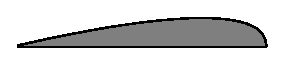
\includegraphics[width=18em]{Pictures/92_PRO13.eps} \vspace{0.5em} \\
Surface:						& As smooth as possible\\
Tuning: 						& Arm 1: positive dihedral 6 - 10 mm; positive angle of attack 1 - 2 mm . Arm 2: positive dihedral 2 - 5 mm; negative angle of attack 0 - 1 mm\\
Wind:							& 1 - 4 Beaufort\\
Throw:							& 5° - 10° angle to the wind, 30° - 50° height of throw, -10° - 20° tilt, throw very hard with lots of spin\\
Flight path:					& A boomerang made of phenolic will fly straight ahead for about 40 m, rises continuously and then lies itself flat. At a height of approx. 25 - 40 metres it reaches the hovering phase and descends slowly\\
Observations:				& It is very difficult to bend and throw a MTA. Beginners should be advised by experienced throwers\\
ATTENTION: 				& MTA boomerangs take up a lot of space and often crash, especially when learning, therefore, make sure that there is nobody on the playing field\\
\end{tabulary}		

\vspace*{\fill}
\begin{center}
	
\includegraphics[width=28em]{plans/PaffIII.eps} 
\end{center}
\vspace{\fill}	

\newpage
\section{Way over the hill}
\begin{tabulary}{30em}{>{\bfseries}lL}
Shape:							& Victor Poulin \\
Use: 								& Sport \\
Flight distance: 			& 50 metres\\
Thickness/material: 	& 5 mm in finnish birch plywood\\
Weight: 						& 96 g / 3.4 oz in wood\vspace{0.5em} \\
Airfoil:							& 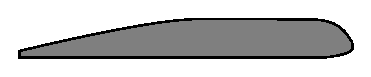
\includegraphics[width=18em]{Pictures/89_PRO10.eps} \vspace{0.5em} \\
Underside:					& Try slight undercut on throwing arm\\
Throw: 							& Throw Hard, approx. approx. 0° height of throw, 15° tilt\\
Wind: 							& 0 - 2 Beaufort  0-8 mph\\
Flight path: 					& Circular, low\\
Tips: 							& If the boomerang is landing out in front of you you can simply twist negative dihedral into the throw arm for 8 seconds and then throw. Or throw when there is wind. Try to use a finger/pistol grib to gain extra spin.\\
\end{tabulary}

\vspace*{\fill}
\begin{center}
	
\includegraphics[angle=90, width=28em]{plans/WayOverTheHill.eps} 
\end{center}
\vspace{\fill}

\newpage
\section{3D Vee}
\begin{tabulary}{30em}{>{\bfseries}lL}
Shape:							& Christoph Schmitz \\
Use: 								& Sport \\
Flight distance: 			& 15-30 metres, depending on size\\
Thickness/material: 	& 3.2mm 3D Printed PLA 6 Perimeters 30\% infill, 3 mm in finnish birch plywood\\
Weight: 						& 25 g / 0.88 oz in PLA\vspace{0.5em} \\
Airfoil:							& 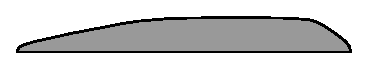
\includegraphics[width=18em]{Pictures/100_PRO21.eps} \vspace{0.5em} \\
Tuning:						& Tape a small coin to arm 1 for more distance \\
Underside:					& Flat, but might benefit from undercut. \\
Weights: 					& Tape a small coin to the lead arm for more distance \\
Throw: 							& 45°-90° angle to the wind, 20°-30° tilt, 5° height of throw\\
Wind: 							& 0 - 3 Beaufort 0-8mph \\
Flight path: 					& Circular, medium height\\
Tips: 							& This boomerang is quite forgiving. The one thing to look out for
			is negative dihedral when it comes off the 3d printer. This needs
			to be corrected to neutral or slightly positive. It can be printed at different sizes; wingspans from 150 mm to 300 mm should work without problems.  May take more if printed densely and/or weighted \\
\end{tabulary}

\newpage
\begin{center}
	\vspace*{\fill}
	
\includegraphics[angle=90, width=28em]{plans/3DVee.eps}
	\vspace*{\fill}
\end{center}

\newpage
\section{Reversible (Windeater 1)}
\begin{tabulary}{30em}{>{\bfseries}lL}
Shape:							& Volker Behrens \\
Use: 								& Sport \\
Flight distance: 			& ?? metres\\
Thickness/material: 	& 5 mm in finnish birch plywood\\
Wingspan:				& ??\\
Weight: 						& ?? g / ?? oz in wood\vspace{0.5em} \\
Airfoil:							& 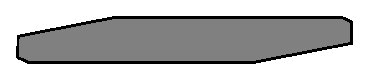
\includegraphics[width=18em]{Pictures/99_PRO20.eps} \vspace{0.5em} \\
Underside:					& This boomerang is reversible so it has a complete airfoil on both sides\\
Throw: 							& Throw Hard with good spin, approx. approx. 10° height of throw, 25° tilt\\
Wind: 							& ?? Beaufort\\
Flight path: 					& Depends on the which side is thrown\\
Tips: 							& Remember when tuning a Reversible - whatever you do affects both boomerangs.\\
\end{tabulary}

\newpage
\begin{center}
	\vspace*{\fill}
	
\includegraphics[angle=0, width=28em]{plans/Reversible.eps}
	\vspace*{\fill}
\end{center}